% This file defines the command for illustrating AMP through a single layer.
% It can be compiled standalone or included in a larger document.

\ifdefined\ispartofbook
\else
  % --- Standalone Compilation Preamble ---
  \documentclass[tikz, border=10pt]{standalone}
  \usepackage{tikz}
  \usetikzlibrary{arrows.meta, positioning}
  \usepackage{amsmath, amssymb} % Added for \vect command
  \newcommand{\vect}[1]{\mathbf{#1}} % Added for \vect command
  \begin{document}
\fi

% --- THE DIAGRAM COMMAND ---
\newcommand{\amplayerdiagram}{%
    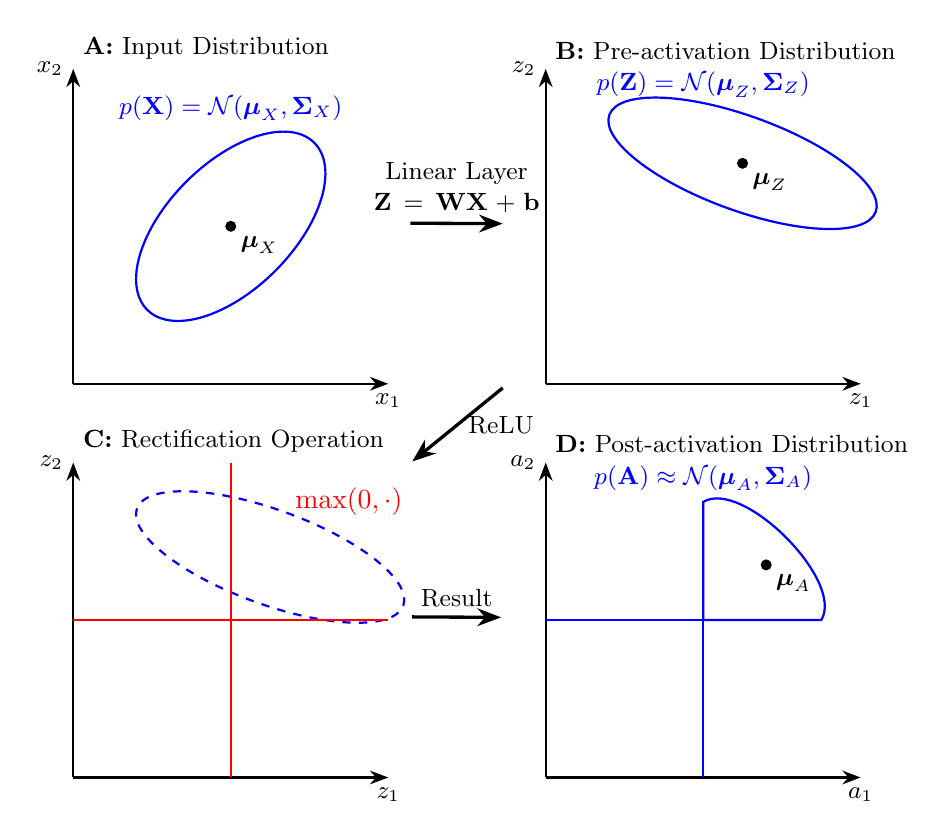
\begin{tikzpicture}[
        font=\sffamily,
        every node/.style={font=\small, align=center}
    ]
    % --- Panel A: Input Distribution ---
    \begin{scope}[local bounding box=panelA]
        \draw[-Stealth, thick] (-2,-2) -- (2,-2) node[below] {$x_1$};
        \draw[-Stealth, thick] (-2,-2) -- (-2,2) node[left] {$x_2$};
        \node[above right] at (-2,2) {\textbf{A:} Input Distribution};
        \draw[blue, thick, rotate around={45:(0,0)}] (0,0) ellipse (1.5cm and 0.8cm);
        \fill[black] (0,0) circle (2pt) node[below right] {$\boldsymbol{\mu}_X$};
        \node[blue] at (0, 1.5) {$p(\vect{X}) = \mathcal{N}(\boldsymbol{\mu}_X, \boldsymbol{\Sigma}_X)$};
    \end{scope}

    % --- Panel B: Linear Transformation ---
    \begin{scope}[local bounding box=panelB, xshift=6cm]
        \draw[-Stealth, thick] (-2,-2) -- (2,-2) node[below] {$z_1$};
        \draw[-Stealth, thick] (-2,-2) -- (-2,2) node[left] {$z_2$};
        \node[above right] at (-2,2) {\textbf{B:} Pre-activation Distribution};
        \draw[blue, thick, rotate around={-20:(0.5,0.8)}] (0.5,0.8) ellipse (1.8cm and 0.6cm);
        \fill[black] (0.5,0.8) circle (2pt) node[below right] {$\boldsymbol{\mu}_Z$};
        \node[blue] at (0, 1.8) {$p(\vect{Z}) = \mathcal{N}(\boldsymbol{\mu}_Z, \boldsymbol{\Sigma}_Z)$};
    \end{scope}

    % --- Panel C: Non-Linear Rectification ---
    \begin{scope}[local bounding box=panelC, yshift=-5cm]
        \draw[-Stealth, thick] (-2,-2) -- (2,-2) node[below] {$z_1$};
        \draw[-Stealth, thick] (-2,-2) -- (-2,2) node[left] {$z_2$};
        \node[above right] at (-2,2) {\textbf{C:} Rectification Operation};
        % Draw original ellipse for context
        \draw[blue, thick, dashed, rotate around={-20:(0.5,0.8)}] (0.5,0.8) ellipse (1.8cm and 0.6cm);
        % Draw axes for rectification
        \draw[red, thick] (-2,0) -- (2,0);
        \draw[red, thick] (0,-2) -- (0,2);
        \node[red, font=\bfseries] at (1.5, 1.5) {$\max(0, \cdot)$};
    \end{scope}

    % --- Panel D: Output Distribution (MODIFIED FOR ALIGNMENT) ---
    \begin{scope}[local bounding box=panelD, xshift=6cm, yshift=-5cm]
        \draw[-Stealth, thick] (-2,-2) -- (2,-2) node[below] {$a_1$};
        \draw[-Stealth, thick] (-2,-2) -- (-2,2) node[left] {$a_2$};
        \node[above right] at (-2,2) {\textbf{D:} Post-activation Distribution};
        % Draw an approximate shape for the rectified distribution, now centered
        \draw[blue, thick] (0,-2) -- (0,0) -- (-2,0); % Boundary axes
        \draw[blue, thick] (0,0) -- (0,1.5) .. controls (0.5,1.8) and (1.8,0.5) .. (1.5,0) -- (0,0);
        \fill[black] (0.8,0.7) circle (2pt) node[below right] {$\boldsymbol{\mu}_A$};
        \node[blue] at (0, 1.8) {$p(\vect{A}) \approx \mathcal{N}(\boldsymbol{\mu}_A, \boldsymbol{\Sigma}_A)$};
    \end{scope}

    % --- Arrows connecting panels ---
    \draw[-{Stealth[length=3mm]}, very thick] (panelA) -- (panelB) node[midway, above, text width=3cm] {Linear Layer \\ $\vect{Z} = \vect{W}\vect{X} + \vect{b}$};
    \draw[-{Stealth[length=3mm]}, very thick] (panelB) -- (panelC) node[midway, right] {ReLU};
    \draw[-{Stealth[length=3mm]}, very thick] (panelC) -- (panelD) node[midway, above] {Result};

    \end{tikzpicture}%
}

\ifdefined\ispartofbook
  % This part is intentionally left blank when included in the main book.
\else
  % This part is for standalone compilation of the image.
  \amplayerdiagram
  \end{document}
\fi
